\chapter{Introduction}
\label{c:intro}
\section{Motivation}
In Standard Model, the decay $B \rightarrow K^{(*)} \nu \bar{\nu}$ are predicted to be highly compressed, the proceed through the flavor-change neutral-current process $b \rightarrow s\nu\bar{\nu}$ are prohibited at tree-level, and it is sensitive to physics beyond the Standard Model. The dominant one-loop box and penguin diagrams are shown in figure \ref{FD}. Theoretical uncertainties on $b \rightarrow s\nu\bar{\nu}$ are predicted smaller than corresponding $b \rightarrow s\ell^+\ell^-$ mode due to the absence of electromagnetic penguin contribution[3]. The effective Hamiltonian for $b \rightarrow s\nu\bar{\nu}$ in SM is\\
\begin{equation}
\label{eq:smt1}
\mathcal{H}^{SM}_{eff} = \frac{4G_F}{\sqrt{2}}V_{tb}V_{ts}^*C^{SM}_L \mathcal{O}_L + h.c.
\end{equation}
\begin{figure}[h]
	\centering
	\subfigure[]{
		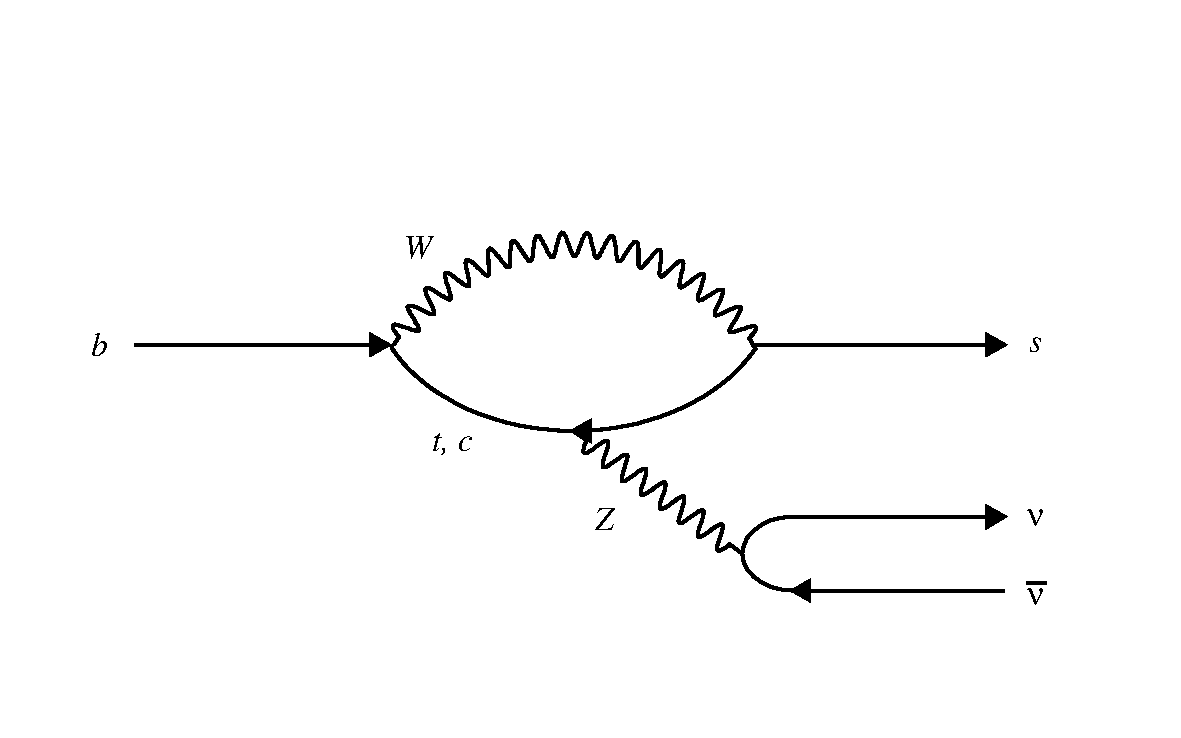
\includegraphics[width=0.45\textwidth]{FeynmanDiagram_hvv_1-eps-converted-to.pdf}
		\label{introduction_figure/FeynmanDiagram_hvv_1}
	}
	\subfigure[]{
		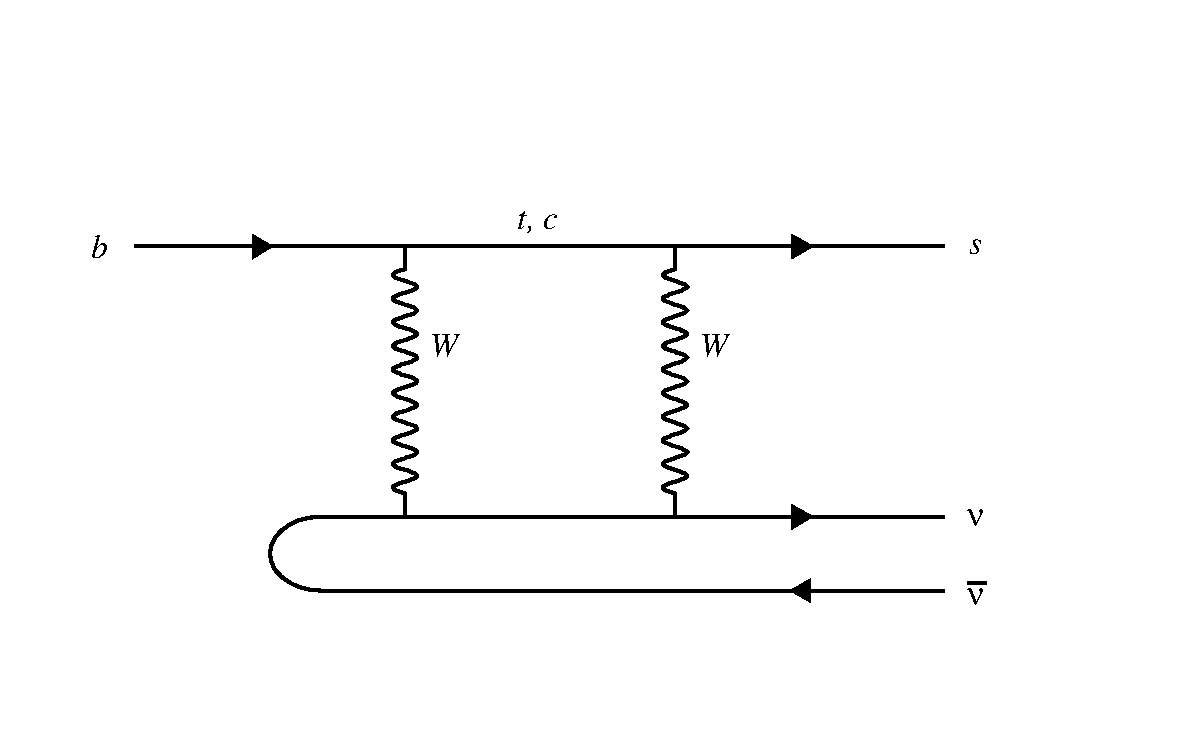
\includegraphics[width=0.45\textwidth]{FeynmanDiagram_hvv_2-eps-converted-to.pdf}
		\label{introduction_figure/FeynmanDiagram_hvv_2}
	}
	
	\caption{Feynman Diagram for $B \rightarrow K^{(*)} \nu \bar{\nu}$ decay }
	\label{FD}	
\end{figure}
\newpage
where
\begin{equation}
\label{eq:smt2}
\mathcal{O}_L = \frac{e^2}{16\pi^2} (\bar{s}\gamma_{\mu}P_L b)(\bar{\nu}\gamma^{\mu}(1-\gamma_5)\nu)
\end{equation}
and $C^{SM}_{L}$ is known as the Wilson coefficient, result in Eq. \ref{eq:smt3}[]
\begin{equation}
\label{eq:smt3}
C^{SM}_{L} = -X_t / s^2_w, ~~~ X_t = 1.469\pm 0.017
\end{equation}
The differential branching ratios as a function of $q^2$, given by [] are


Here, the factor of 3 stems from the total neutrino flavour, $N$ stand for a normalization factor shown in Eq. \ref{eq:smt6}, $\rho_i$ are  rescaled form factors shown in Eq. \ref{eq:smt6} $\sim$ \ref{eq:smt10}.
\begin{equation}
\label{eq:smt6}
N = V_{tb}V_{ts}^*\frac{G_F \alpha}{16 \pi ^2} \sqrt{\frac{m_B}{3 \pi}}
\end{equation}
\begin{equation}
\label{eq:smt7}
\rho_V(q^2) = \frac{2q^2 \lambda^{3/2}_{K^*}(q^2)}{(m_B + m_{K^*})^2 m_B^4}[V(q^2)]^2
\end{equation}
\begin{equation}
\label{eq:smt8}
\rho_{A1}(q^2) = \frac{2q^2 \lambda^{1/2}_{K^*}(q^2)(m_B + m_{K^*})^2}{ m_B^4}[A_1(q^2)]^2
\end{equation}
\begin{equation}
\label{eq:smt9}
\rho_{A12}(q^2) = \frac{64m^2_{K^*}\lambda^{1/2}_{K^*}(q^2)}{m_B^2}[A_{12}(q^2)]^2
\end{equation}
\begin{equation}
\label{eq:smt10}
\rho_K(q^2) = \frac{\lambda^{3/2}_{K}(q^2)}{m_B^4}[f^K_+(q^2)]^2
\end{equation}
which the 
\begin{equation}
\label{eq:smt11}
\lambda (a,b,c) = a^2+b^2+c^2-2(ab+bc+ac), \lambda^{3/2}_{K}(q^2) \equiv \lambda(m^2_B, m^2_K{(*)}, q^2)
\end{equation}
The SM branching ratio estimate to be $\mathcal{B}(B^+ \rightarrow K^{+} \nu \bar{\nu})=\mathcal{B}(B^0 \rightarrow K^{0} \nu \bar{\nu}) = (4.5 \pm 0.7) \times 10^{-6}$, $\mathcal{B}(B^+ \rightarrow K^{*+} \nu \bar{\nu})=\mathcal{B}(B^0 \rightarrow K^{*0} \nu \bar{\nu}) = (6.8 ^{+1.0}_{-1.1}) \times 10^{-6}$.\\

There are many new-physics models predicted that could significantly enhance the branching ratio, as well as modify the expected SM $S_B$ distributions, where $S_B \equiv q^2/m^2_B$, $q^2$ is the square magnitude of missing four-momentum as the neutrino pair, $m_B$ is the B meson mass. Some of these models predict that some massive particle could contribute extra loop diagrams with similar amplitudes as those in SM, like nonstandard $Z^0$ couplings with SUSY(supersymmetric) particle, fourth generation quarks, anomalous top-charm transitions, and a massive U(1) gauge boson $Z^{'}$. There are others thing that can do some contribution, such like the missing part of the nrutrino pair can be replaced as the low-mass dark mass or right-handed neutrino candidate, the kaon can be replaced as the SUSY particles.\\
This analysis $B \rightarrow K^{(*)} \nu \bar{\nu}$ is measure several times by both BaBar and Belle experiment, with the current data, there were no signal observed, but was very close to see it. In this thesis, our goal is to do the enhancement on signal efficiency in the previous study at Belle\cite{ref:Lutz2013}, and do the bin-by-bin optimization on $S_B$ distribution, because certain new-physics models imply that enhancements are possible at high $S_B$ region, instead of removing the low $S_B$ region in the previous study, we measure the partial branching fraction$(\Delta \mathcal{B})$ in the interval of $S_B = 0.1$.\\
We also perform the measurement result in pseudo Belle II data, which times the factor of 50 in both signal Monte Carlo and background Monte Carlo, with the Belle II experiment in the future, the luminosity will increasing by the factor of 50, this gives us the chance to probe the new physics models through such kind of these decay mode like $B \rightarrow K^{(*)} \nu \bar{\nu}$.

\section{Standard Model}
The Standard Model (SM) is a relativistic quantum field theory that describing the interactions between the elementary particle. In Standard Model, four families of the elementary particle and also it antiparticle are include, there are six kinds of quarks, six kinds of leptons, four kinds of gauge bosons and the Higgs boson.The Standard Model is also describes all known forces, electromagnetic force, weak force, and strong force. Only gravity is not include in Standard Model. Figure \ref{Standard_Model_of_Elementary_Particles} shows all the element and their corresponding properties in Standard Model, and Figure \ref{Elementary_particle_interactions} shows the interaction between the elementary particle in SM.\\

\begin{figure}[h]
		\centering
		\subfigure[Standard Model of Elementary Particles.]{
			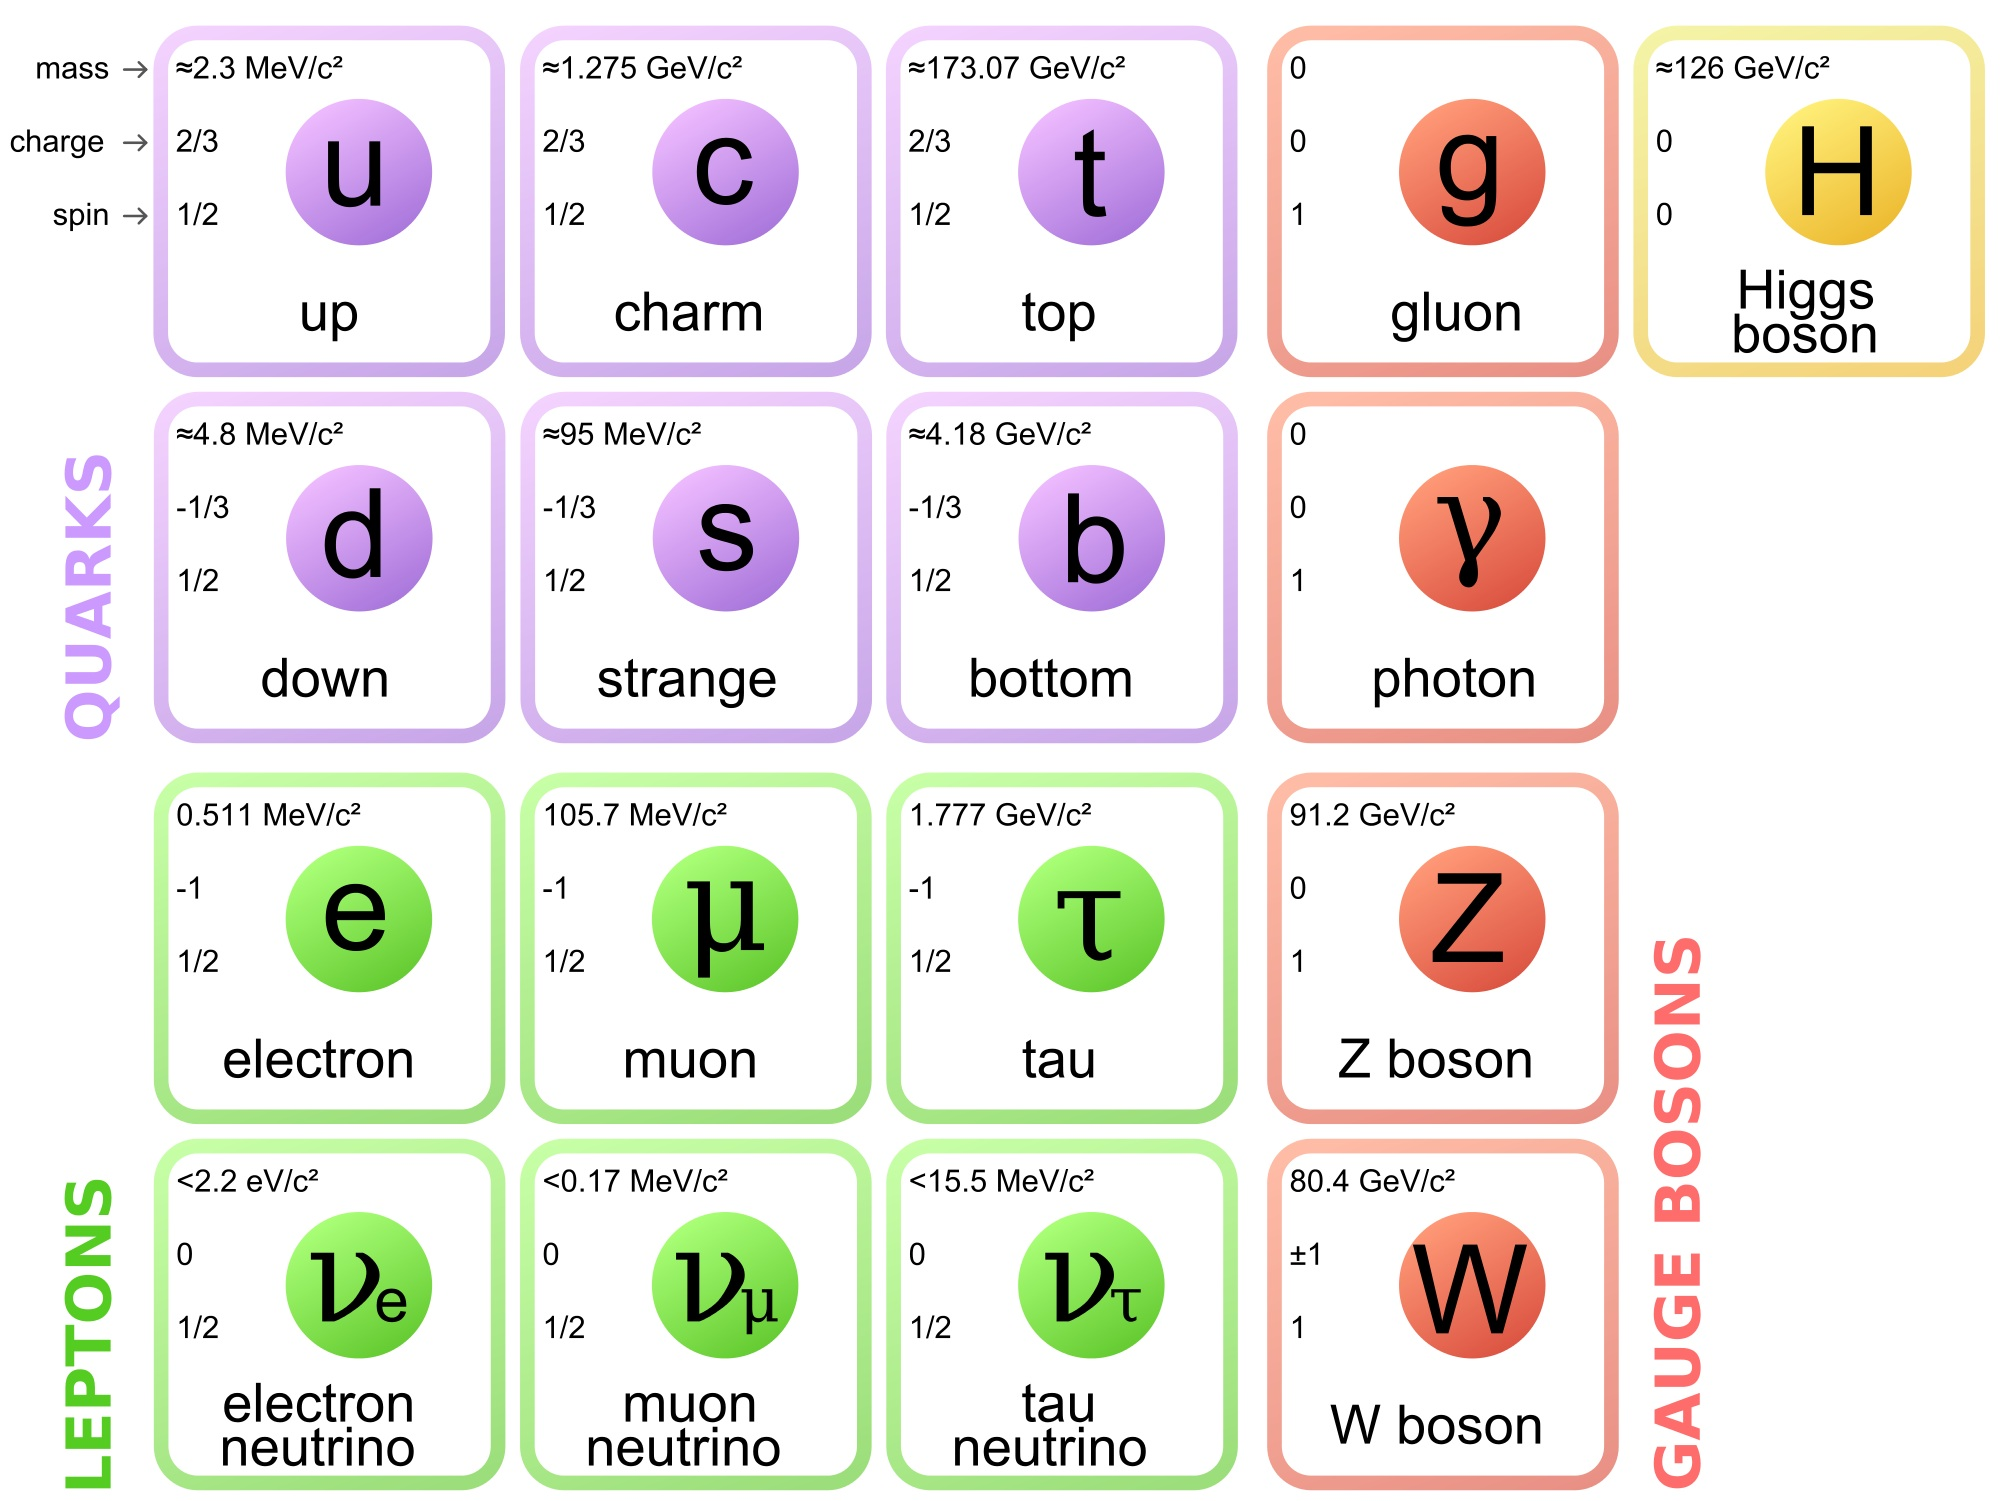
\includegraphics[width=0.45\textwidth]{Standard_Model_of_Elementary_Particles}
			\label{introduction_figure/Standard_Model_of_Elementary_Particles}
		}
		\subfigure[The interactions between elementary particle of the Standard model.]{
			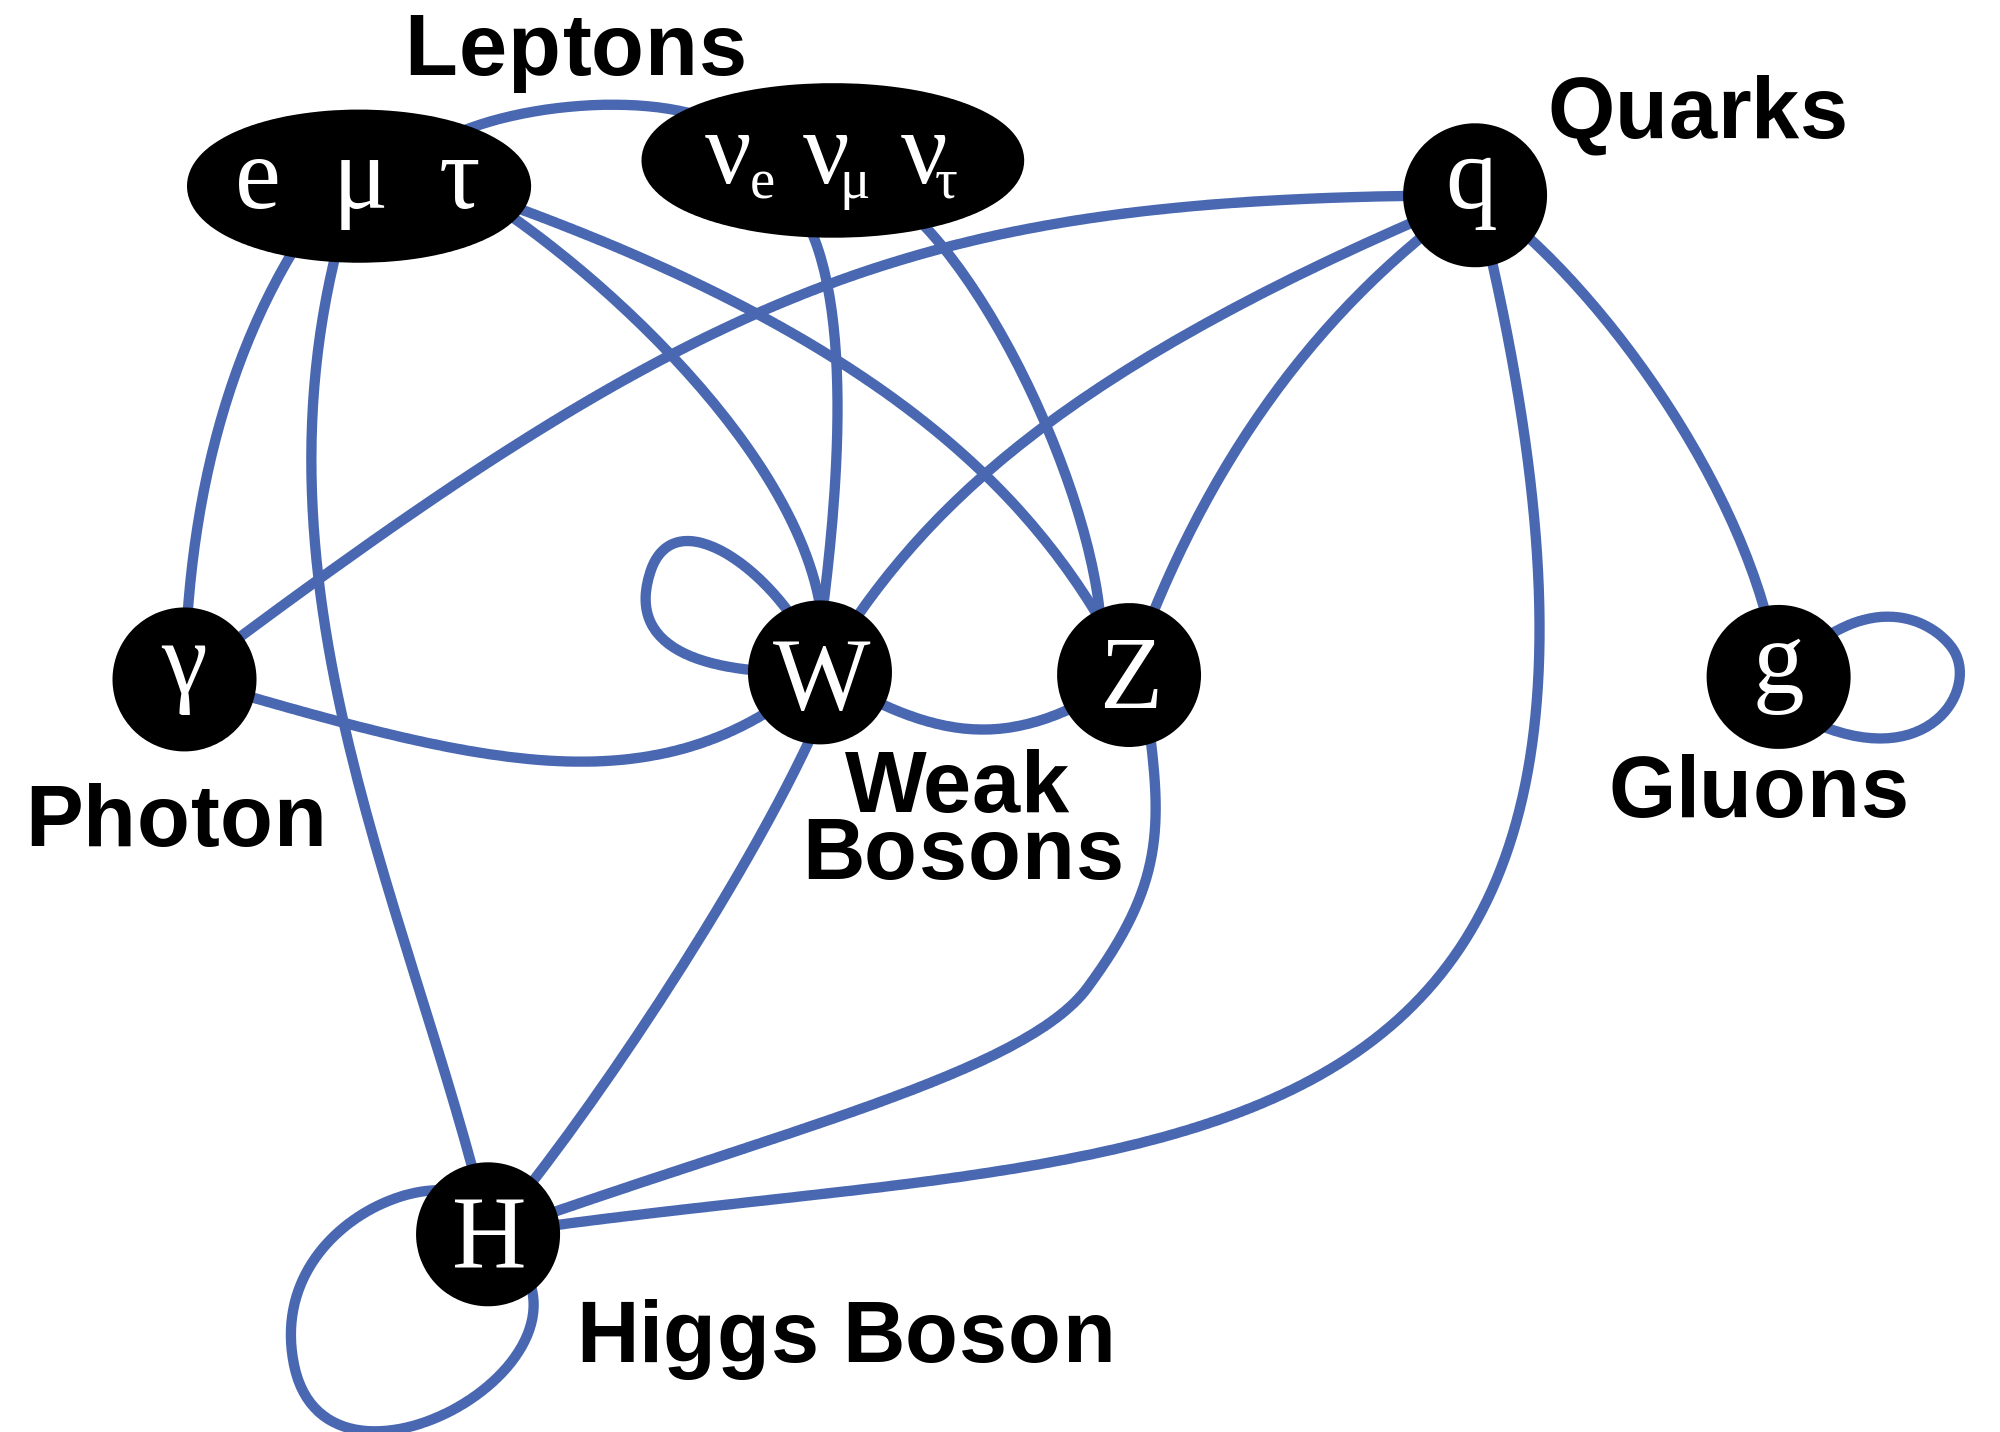
\includegraphics[width=0.45\textwidth]{Elementary_particle_interactions}
			\label{introduction_figure/Elementary_particle_interactions}
		}
		\label{SM}	
		\caption{fuck}

\end{figure}

Mathematically, the Standard Model is formed by the local gauge symmetry $SU$(3) $\times$ $SU$(2) $\times$ $U$(1). The $SU$(3) represents the strong force and only particle can interact strongly, The $SU$(2) is stand for weak interaction, and only the particle in weak doublets can interaction through weak force and electromagnetic force is described by $U$(1) symmetry with the weak hyper-charge.


\subsection{Elementary Particle}
\begin{table}[h]
\begin{center}
\begin{tabular}{l|c|c|c|c|c|c|c|c|r}
\hline
\hline
			Quark   &  Mass(Mev/$c^2$)   	&   J     &    B      &   Q    &    $I_3$   &   T      &   S    &   C   &	$B^{'}$   \\
\hline
			  $u$      & 2.3    	&   1/2     &  +1/3        &   +2/3    &   +1/2    &    0     &   0    &   0   &0	   \\
\hline
			  $d$     &  4.8   	&     1/2    &     +1/3      &   -1/3    &    -1/2   &    0     &   0    &   0   &	0   \\
\hline
			 $c$      &   1275  	&    1/2     &    +1/3       &   +2/3    &   0    &    0     &  0     &  +1    &0	   \\
\hline
			 $s$		&  95   	&   1/2      &    +1/3       &   -1/3    &   0    &    0     &   -1    &    0  &0	   \\
\hline
			 $t$		&   173210  	&   1/2      &   +1/3        &   +2/3    &  0     &   +1      &   0    &  0    &0	   \\		
\hline
			 $b$		&  4180   	&   1/2      &     +1/3      &   -1/3    &  0     &     0    &   0    &  0    &	-1   \\		
\hline
\hline						        
\end{tabular}
\caption{ Some quantum number of the six quarks\\J = total angular momentum, B = baryon number, Q = electric charge, I3 = isospin, C = charm, S = strangeness, T = topness, B′ = bottomness.} \label{t:quarka}
\end{center}
\end{table}

\subsection{The Cabibo-Kobayashi-Maskawa Matrix}


\subsection{B physics}
In 1977,the third generation bottom quark(b) was observed by the CFS\footnotemark[1]
E288 experiment headed by Leon Lederman at Fermi lab. 
A dimuon resonance at 9.5 GeV was found,which now recognized as $\Upsilon$ (1S).
$\Upsilon$ is a flavorless meson formed by a b quark and an anti-b quark. Figure 1.3 shows
the cross section to particle production of various $\Upsilon$ states measured by CUSB$\footnotemark[2]$
and CLEO detector in CESR$\footnotemark[2]$ at Cornell University.
B mesons are the
\footnotetext[1]{Columbia-Fermilab-Stony Brook colla}
\footnotetext[2]{Ego's id is mapped by Appendix}
\subsection{CP Violation}

%\begin{table}[t]
%\begin{center}
%\begin{tabular}{lcc}
%
%\hline
%                    &  {\small Itti's method}     & {\small Fuzzy growing}    \\
%\hline
%{\small Precision}           &  0.4475    & 0.4506 \\
%{\small Recall}              &  0.5515    & 0.5542 \\
%\hline
%
%\end{tabular}
%\caption[Evaluation of FOA sets]{\small Evaluation of FOA sets. } \label{t:FOA}
%\end{center}
%\end{table}
